\chapter{Guía de instalación y puesta en marcha de BreachLab}
\label{anexo:instalacion}

Este anexo recoge los pasos necesarios para desplegar \breachlab y
reproducir las pruebas descritas en el capítulo~\ref{cap:explotacion}.

\section{Despliegue con Docker (recomendado)}

\begin{console}
cd tfm-lab
docker compose up --build
# Abre http://localhost:8080
\end{console}

\begin{figure}[htbp]
  \centering
  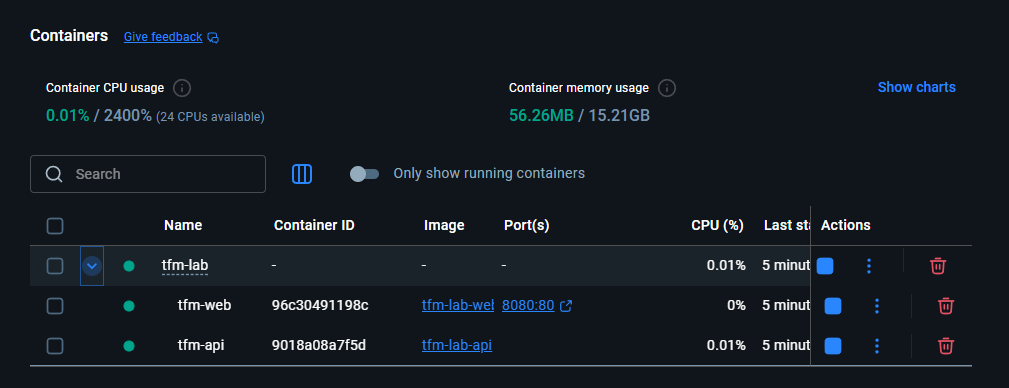
\includegraphics[width=0.85\textwidth]{figures/docker-containers.png}
  \caption{Los dos contenedores de \breachlab (\texttt{tfm-web} y
    \texttt{tfm-api}) en ejecución tras \texttt{docker compose up --build},
    vistos desde Docker Desktop.}
  \label{fig:docker-containers}
\end{figure}

\section{Despliegue en modo desarrollo (dos terminales)}

\begin{console}
# Terminal 1: backend
cd tfm-lab/backend
pip install -r requirements.txt
python api.py                      # API en http://localhost:5000

# Terminal 2: frontend
cd tfm-lab/frontend
npm install
npm run dev                        # Front en http://localhost:4321
\end{console}

\section{Usuarios de prueba}

\texttt{admin} / \texttt{Admin123!} (rol admin), \texttt{marina} /
\texttt{contraSegura} (rol user) y \texttt{pablo} / \texttt{qwerty} (rol
user). El enlace «Reiniciar base de datos» de la página de inicio (o
\texttt{GET /api/reset}) devuelve la base de datos a su estado inicial.

\section{El interruptor \texttt{?safe=1}}

Añadido a la URL de cualquier página, activa a la vez las contramedidas de
frontend y de backend correspondientes. El badge de la barra superior de la
aplicación indica en todo momento el modo activo.
